% newcommands, defined by fracapuano (feel free to move them wherever is more appropriate)
\newcommand{\actionchunk}{\mathbf{A}}
\newcommand{\actionexpert}{\mathbf{v}_\theta}

\section{SmolVLA: small, efficient and capable}

\paragraph{Overview.}
\ours is a lightweight VLA composed of a compact pretrained VLM, and an action expert trained with flow matching. 
Given multiple images and a language instruction describing the task, the model outputs a chunk of actions. 
It is first pretrained with imitation learning on community-collected datasets, then evaluated across both real-world and simulated environments. 
The pretraining data is designed to span a diverse set of tasks and behaviors, allowing the model to learn generalizable physical skills that transfer across settings. 
At inference time, we introduce an asynchronous execution stack that decouples action execution from perception and prediction, enabling faster and more responsive control.

\subsection{Model architecture}
SmolVLA is composed of two main components: \emph{(i)} a pretrained VLM tasked with perception and \emph{(ii)} an action expert, trained to act. 
The two components are interconnected, as the VLM processes state inputs to generate features that condition the action expert, which produces actions in turn altering the state fed to the VLM. 
Specifically, the VLM processes sensorimotor states, including images from multiple RGB cameras, and a language instruction describing the task. In turn, the VLM outputs features directly fed to the action expert, which outputs the final continuous actions.

\paragraph{Vision-language model (VLM).}
We leverage a pretrained VLM as the main backbone for perceiving the robot’s environment. VLMs, pretrained on diverse multimodal data, capture rich world knowledge. To guarantee efficiency and accessibility, we choose SmolVLM-2~\citep{marafioti2025smolvlm}, an efficient model optimized for multi-image and video inputs. 
SmolVLM-2 relies on SigLIP~\citep{li2023siglip} to encode visual features for SmolLM2 language decoder~\citep{allal2025smollm2}.
In \ours, the VLM component processes image sequences using the vision encoder, which reduces token count through a token-shuffling technique for efficiency. The language instruction is tokenized into text tokens. Sensorimotor states are projected into a single token via a linear layer to match the language model’s token dimension. Lastly, visual, language, and state tokens are concatenated and passed to the language decoder. The resulting obtained via the decoder layers are then used to condition the action expert.

\paragraph{State, action, and feature projectors.}
We use linear projection layers in various points inside of \ours. In particular, we use linear projection layers to \emph{(i)} project the states to match the VLM dimension \emph{(ii)} project the actions to match the action expert dimensions and \emph{(iii)} to adapt the VLM features to align with the action expert’s dimension.

\paragraph{Visual tokens reduction.}
While proven critical for VLM performance, high-resolution images increase inference costs. 
To guarantee efficiency, SmolVLM-2 is trained with image tiling~\citep{lin2023sphinx}, a popular technique that involves processing multiple crops of the same image, in addition to the global image. 
However, to obtain a faster inference time, we do not use tiling. We use the global image only, in addition to a pixel shuffle operation, limiting the visual tokens to 64 per frame.

\paragraph{Faster inference through layer skipping.}
To get faster inference time, we skip computations in the VLM. Prior work~\citep{shukor2024skipping,tang2023you} demonstrated the possibility of skipping layers in pretrained models without incurring in significant performance degradation. 
Recently,~\citep{el2024scalable,bolya2025perception,rajasegaran2025empirical} have shown that the best features for downstream tasks are not necessarily obtained from the last layer of a VLM. 
Consequently, rather than using the last layer features, our action expert has access to all features up to a specified layer \( N \). 
In practice, we find setting \( N \) to half the total layers (\( N=L/2 \)) offers a good tradeoff between speed and performance, effectively halving the LLM and action expert’s computational cost.

\paragraph{Flow matching action expert.}
The action expert \( \mathbf{v}_{\theta} \) is trained to predict an action chunk \( \actionchunk_t = ( a_t, \ldots, a_{t+n} ) \) from VLM features.
In keeping with prior work, our implementation of \( \mathbf{v}_\theta \) relies on the transformer architecture \citep{vaswani2017attention}.
Differently from prior VLA architectures, we interleave cross and self-attention layers, thus using a conditional Flow Matching Transformer~\citep{esser2024scaling,liu2022rectified,lipman2022flow} as \(  \mathbf{v}_{\theta} \). 
The action expert is trained using the objective defined by:

\begin{equation*}
\mathcal L ^\tau(\theta) = \mathbb{E}_{p(\actionchunk_t \mid \mathbf{o}_t), q(\actionchunk_t^\tau \mid \actionchunk_t)} \left[ \left\| \mathbf{v}_{\theta}(\actionchunk_t^\tau, \mathbf{o}_t) - \mathbf{u}(\actionchunk_t^\tau \mid \actionchunk_t) \right\|^2 \right],
\end{equation*}

where $\mathbf{o}_t$ represents the VLM features extracted from an observation \( o_t \) at the \( N \)-th VLM layer, and \( \actionchunk_t^\tau = \tau \actionchunk_t + (1 - \tau) \epsilon \), with \( \epsilon \sim \mathcal{N}(0, \mathbf{I}) \). 
In particular, \( \mathbf{v}_{\theta} \) is trained to output the vector field \( \mathbf{u}(\actionchunk_t^\tau \mid \actionchunk_t) = \epsilon - \actionchunk_t \) from the VLM features and the noisy actions \( \actionchunk_t^\tau \). 
In keeping with~\citet{black2024pi_0}, we sample \( \tau \) from a Beta distribution. To improve on inference's efficiency, we use a reduced hidden size of \( 0.75 \times d \) for \( \mathbf{v}_\theta \), where \( d \) is the VLM's hidden dimension.

\paragraph{Interleaved cross and causal self-attention layers.}
The action expert \( \actionexpert \) generates action chunks conditioned on the VLM features, with the interaction between the VLM and action expert in \ours being facilitated by the attention mechanisms.
Unlike prior works relying exclusively on self-attention (SA)~\citep{black2024pi_0} or cross-attention (CA)~\citep{bjorck2025gr00t}, we employ an interleaved approach, where each block contains either a CA or a SA layer. 
This design choice also differs from standard VLM architectures, where each decoder block typically includes both SA and CA layers~\citep{OBELICS,alayrac2022flamingo,chen2022pali}. 
Within the action expert's forward pass, the interaction between actions and VLM features takes place via attention, projecting tokens into query, keys and values~\citep{vaswani2017attention}. 
In our setup, CA layers cross-attend the VLM's keys and values, while SA layers allow the action tokens in \( \actionexpert \) to attend to each other.
We employ a causal attention mask for the SA layers, ensuring that each action token can only attend to past tokens within the chunk, preventing future action dependencies. Empirically, we find that interleaving CA and SA layers provides higher success rates and faster inference time. In particular, we find self-attention to contribute to smoother action chunks \( \actionchunk \), something particularly evident when evaluating on real robots.

% \subsection{More efficient VLA architecture}

% \paragraph{No attention on actions.} causal vs bidir vs cross

% \paragraph{Skipping computations}

% \paragraph{Less visual tokens.}

% \paragraph{States to prefix.} Flow matching steps on less tokens.

% \paragraph{Efficient Training and Data Loading.}
% Beyond maintaining a compact model and a reduced number of tokens, we employ several optimizations to enhance training efficiency. Specifically, we leverage bfloat16 precision and torch.compile() \citep{paszke2019pytorch} that JIT-compiles PyTorch code into optimized kernels. To ensure compatibility with these optimizations, we maintain a fixed sequence length and  batch size, discarding any excess frames in an episode that do not fit a complete batch. For multi-GPU and multi-node training, we utilize Hugging Face accelerate \citep{accelerate} library with mixed precision, providing a scalable and memory-efficient training setup. 

% \Mus{Data loading efficiency tricks.}

% \section{Training data}

% \begin{comment}
% GR00T \cite{bjorck2025gr00t} mitigates the “data island” problem by structuring training data as a three-tiered pyramid—combining large-scale web and human videos, synthetic simulations, and real-world robot data—and applying a unified co-training strategy across these heterogeneous sources using latent action modeling and inverse dynamics prediction.   
% \end{comment}

% \subsubsection{Academic datasets.}

\subsection{Pretraining data collected by the community}

In robotics, the data available for large-scale pretraining remains orders of magnitude smaller than what has driven recent breakthroughs in vision and language. 
For instance, while natural language foundation models can benefit from the unique text-based interface and massive scale of internet-data, the integration and scaling up of robotics datasets appears complex, due to the \emph{(i)} differences across datasets and \emph{(ii)} reliance on teleoperation by human experts for data collection.
Additionally, the high heterogeneity of robot morphologies, sensors, actuation modes, control frequencies, and data formats results in "data islands"~\cite{bjorck2025gr00t}--scattered robotics datasets whose integration proves challenging.

In this context, the advent of low-end robotic platforms and standardized robotics libraries directly mitigates this data heterogeneity, providing a unique entry point to robotics for practitioners. 
Further, open-source data contributions collected by individual practitioners enable the larger robotics community with \textit{community datasets}, datasets collected in diverse real-world settings--from academic labs to homes--as part of a larger effort to decentralize and scale robot learning with open-source.
Unlike academic datasets following standardized protocols, community datasets naturally span varied robot embodiments, control schemes, camera perspectives, and tasks. Further, community datasets reflect real-world complexity through noisy demonstrations, heterogeneous environments, and diverse object interactions, providing valuable as pre-training data. In this work, we selected a subset of 481 community datasets obtained from Hugging Face, filtered according to embodiment type, episode count, overall data quality, and frame coverage (Table~\ref{tab:pretraining_data}).


% making them well-suited for pretraining generalist robot policies.

% The resulting pretraining mixture includes 481 datasets collected with So100 arms.


% Community datasets, in this context, refer to datasets contributed by practitionners and shared on the Hugging Face Hub under the lerobot tag; these are subsequently termed LeRobot Community Datasets. These datasets are recorded in diverse environments—ranging from academic labs to homes—and represent a decentralized, open-source effort to scale real-world robot data collection.

% In contrast to large academic datasets, which often follow specific protocols, LeRobot Community Datasets naturally cover a growing spectrum of robot embodiments, control schemes, camera viewpoints, and task types. They reflect real-world complexity through imperfect demonstrations, heterogeneous environments, varied lighting conditions, and unconventional object interactions. This variability aligns directly with the goals of pretraining, making community datasets not only a critical complement to academic corpora but potentially a standalone foundation for generalist robot learning. 

% The current LeRobot community datasets used in this work comprise around \Dana{add number} datasets. These datasets have undergone a thorough filtering process based on several criteria, including the number of frames, type of embodiment, qualitative assessment of the frames, and number of episodes. As a result, the dataset collection was refined to a final training mixture containing around 481 datasets with SO100 arms.

\vspace{-0.4cm}
\begin{wraptable}{r}{0.4\linewidth}
    \centering
    \setlength{\tabcolsep}{8pt} % Adjusted for compactness
    \renewcommand{\arraystretch}{1} % Improved row spacing
    \resizebox{\linewidth}{!}{
        \begin{tabular}{ccccccc}
            \toprule
            \textbf{\# datasets} & \textbf{\# episodes} & \textbf{\# frames}  \\
              481 & 22.9K & 10.6M\\
            \bottomrule
        \end{tabular}
    }
    \captionof{table}{\textbf{Community datasets statistics.} At \(\sim\) 10M episodes, our pretraining set stands at least one order of magnitude smaller than other state-of-the-art. For completeness, we report the list of community-datasets used in \Cref{app:comm_data}.}
    \vspace{-0.4cm}
    \label{tab:pretraining_data}
\end{wraptable}

\paragraph{Task annotation with VLM.} 
Relying on community-contributed datasets entails standardization challenges. In particular, we observed substantial noise in task annotations--natural language descriptions of the robot’s intended behavior for a given dataset. 
Critically, various datasets included ambiguous placeholders such as \texttt{task desc}, overly vague commands such as \texttt{Hold} or \texttt{Up}, or lacked instructions entirely. To improve on the annotation quality, we used an off-the-shelf VLM (\texttt{Qwen2.5-VL-3B-Instruct}) to auto-generate concise task descriptions. For each dataset, we sampled representative frames and provided them alongside the original instruction. The model was prompted to produce a short, action-oriented sentence summarizing the behavior. The full prompt is available in \Cref{app:comm_data}.

\paragraph{Camera viewpoint normalization.} 
Another challenge arising from using community datasets consists in the high variability in the camera naming conventions used. For instance, datasets refer \texttt{images.laptop} may refer to a top, side, or wrist-mounted view depending on the particular. We found this inconsistency detrimental during pretraining, and that a consistent camera ordering is rather beneficial for training in this data regime. To address this standardization challenge, we manually mapped each camera to a standardized view type—prioritizing top, wrist, and side perspectives--and renamed them as \texttt{OBS\_IMAGE\_1}, \texttt{OBS\_IMAGE\_2}, and \texttt{OBS\_IMAGE\_3}, respectively. 
For datasets with additional views, the order was preserved, but unused views were dropped during training. Future efforts may automate this process using VLMs, or propose/adopt standardized data collection guidelines.

% Automatically inferring these viewpoints is error-prone and negatively impacted model performance on practice.

% Ideally, features like \texttt{images.laptop} correspond to a top-down view, while \texttt{images.iphone} represents a wrist-mounted or side view. Some datasets adopt clearer naming conventions, explicitly labeling views such as \texttt{right}, \texttt{left}, \texttt{top}, \texttt{bottom}, or \texttt{wrist.right}, \texttt{wrist.top} and etc. 

% However, ambiguous labels are common. For example, \texttt{images.laptop} can refer to either a third-person view or a wrist-level camera, depending on the dataset. Automatically inferring these viewpoints is error-prone and negatively impacted model performance on practice.

% To address this, we manually reviewed and mapped each camera perspective to a standardized naming scheme (e.g., ensuring that \texttt{top} corresponds to an actual top-down view). During training, all image features were uniformly renamed as \texttt{OBS\_IMAGE\_1}, \texttt{OBS\_IMAGE\_2} and \texttt{OBS\_IMAGE\_3} for the top, wrist and side camera views respectively, for datasets with additional viewpoints. In the future, this task could be automated using vision-language models or computer vision classifiers to classify and standardize camera perspectives more efficiently, or by following a standardized guideline or checklist during data recording that we shared with the community.

\subsection{Asynchronous inference}\label{sec:async}

Modern visuomotor policies~\citep{zhao2023learningact, chi2023diffusion, black2024pi_0} output \emph{action chunks}--sequences \(\pi(o_t) = \actionchunk_t \) with \(\actionchunk_t = \bigl(a_t,a_{t+1},\dots,a_{t+n}\bigr) \) being a sequence of \(n \) (much greater than 1) low-level commands enqueued in an action queue, originating from an environment observation, \(o_t\).
Typically, the robot executes the entire action chunk \(\actionchunk_t \), before a new observation \( o_{t+n} \) is passed to the policy \( \pi \) to predict the next chunk. This results in open-loop inference in between observations captured every \( n \) timesteps.
Works including~\citet{zhao2023learningact, chi2023diffusion} adopt a different strategy whereby the robot controller interleaves chunk prediction \( \actionchunk_t \gets \pi(o_t) \) and chunk consumption \( a_t \gets \textsc{PopFront(\( \actionchunk_t \))} \), computing a new chunk of actions at every timestep \( t \) and aggregating the predicted chunks on overlapping sections.
While adaptive--every observation at every timestep \( o_t\) is processed--such approaches rely on running inference continuously, which can be prohibitive in resource-constrained scenarios, such as edge deployments.

A less resource-intensive approach is to entirely exhaust the chunk \( \actionchunk \) before predicting a new chunk of actions, a strategy we refer to as \textit{synchronous} (sync) inference. 
Moreover, sync inference efficiently allocates computation every \( n \) timestep, resulting in a reduced average computational burden at control time. In contrast, it inherently hinders the responsiveness of robot systems, introducing blind lags due to the robot being \textit{idle} while computing \( \actionchunk \).

We directly assess the lack of adaptiveness of robot systems due to acting open-loop, and the presence of lags at runtime by decoupling action chunk prediction \( \actionchunk \) from action execution \( a_t \gets \textsc{PopFront}(\actionchunk_t) \), developing an \textit{asynchronous} (async) inference stack (\Cref{alg:async-inference}), whereby a \( \textsc{RobotClient} \) sends an observation \( o_t \) to a \( \textsc{PolicyServer} \), receiving an action chunk \( \actionchunk_t \) once inference is complete (\Cref{fig:async-inference}).
In this, we avoid execution lags by triggering chunk prediction while the control loop is still consuming a previously available queue, aggregating it with the newly incoming queue whenever available.
In turn, async-inference tightens the loop between action prediction and action execution, by increasing the frequency at which observations are processed for chunk prediction. 
Crucially, decoupling action prediction from action execution also directly allows to allocate more computational resources on a remote policy server sending actions to the robot client over networks, something which may prove very effective in resource-constrained scenarios such as low-power robots.

\begin{figure}
    \centering
    \begin{minipage}[t]{\textwidth}
        \centering
        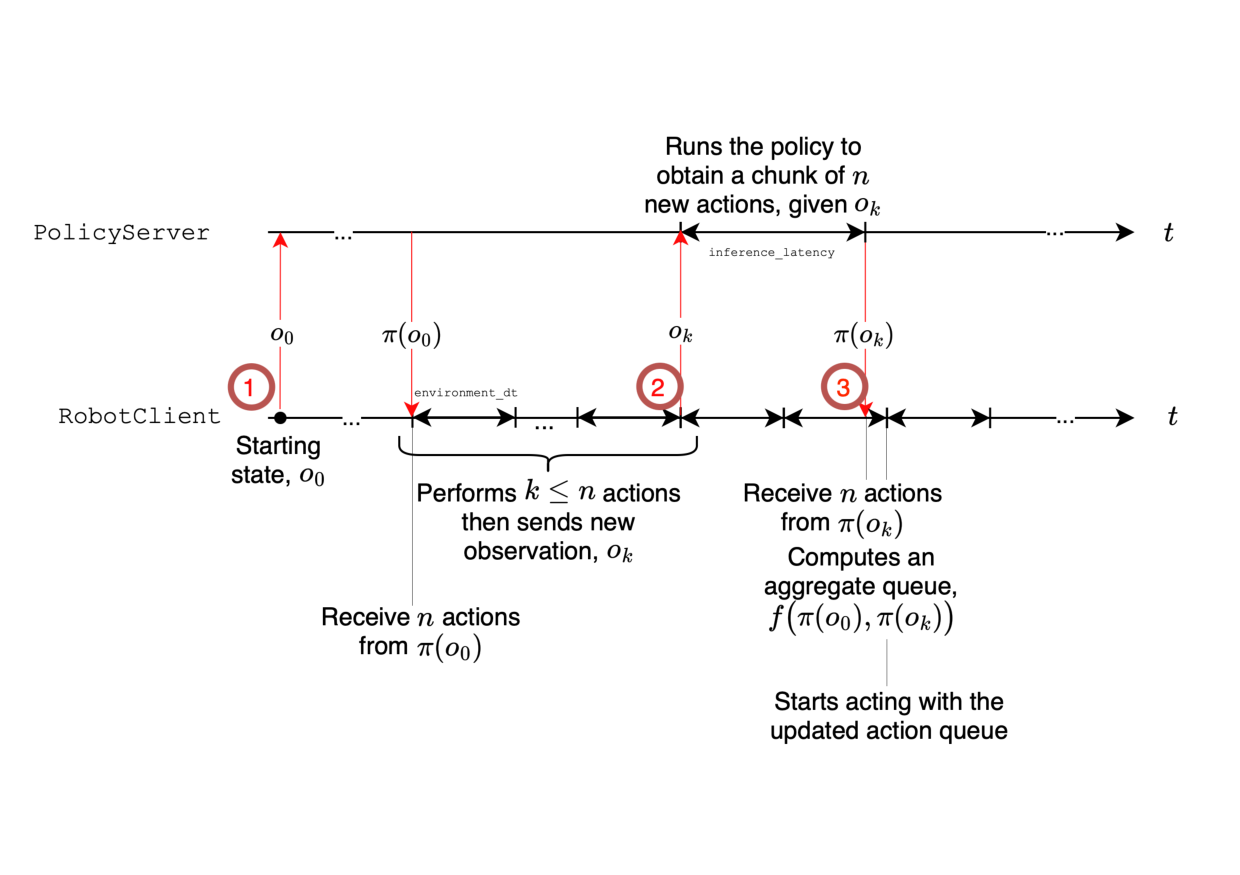
\includegraphics[width=0.9\textwidth]{figures/async_inference.pdf}
        \caption{\textbf{Asynchronous inference}. Illustration of the asynchronous inference stack. Note that the policy can be run on a remote server, possibly with GPUs.}
        \label{fig:async-inference}
    \end{minipage}
    \vspace{-0.6cm}
\end{figure}

\begin{algorithm}
  \caption{Asynchronous inference control-loop}
  \label{alg:robotclient}
  \begin{algorithmic}[1]
    \State \textbf{Input:} horizon $T$, chunk size $n$, threshold $g\in[0,1]$
    \State \textbf{Init:} capture $o_0$; send $o_0$ to \textsc{PolicyServer};
           receive $\actionchunk_0 \gets \pi(o_0)$
    \For{$t$ \textbf{to} $T$}
        \State $a_t \gets \textsc{PopFront}(\actionchunk_t)$
        \State \textsc{Execute}($a_t$) \Comment{execute action at step $t$}
        \If{$\tfrac{|\actionchunk_t|}{n} < g $} \Comment{queue below threshold}
            \State capture new observation, $o_{t+1}$
            \If{\textsc{NeedsProcessing}$(o_{t+1})$} \Comment{similarity filter, or triggers direct processing}
                \State \texttt{async\_handle} $\gets \textsc{AsyncInfer}(o_{t+1})$ 
                \Comment{Trigger new chunk prediction (non blocking)}
                \State $\tilde{\actionchunk}_{t+1} \gets \pi(o_{t+1})$ \Comment{New queue is predicted with the policy}
                \State $\actionchunk_{t+1} \gets f(\actionchunk_t,\tilde{\actionchunk}_{t+1})$ \Comment{aggregate overlaps (if any)}
                
            \EndIf
        \EndIf
        \If {\textsc{NotCompleted}(\texttt{async\_handle})}
            \State $\actionchunk_{t+1} \gets \actionchunk_t$ \Comment{No update on queue (inference is not over just yet)}
        \EndIf
    \EndFor
  \end{algorithmic}
  \label{alg:async-inference}
\end{algorithm}


\paragraph{Implementation details}
% The proposed \textit{async} stack decouples \emph{action prediction} from \emph{action execution}, allowing inference to overlap with control.
\textit{Async} inference \emph{(i)} tightens the control loop by capturing observations more often, directly eliminates idle gaps at runtime, and \emph{(ii)} directly allows to run inference on more powerful computational resources than the ones typically available onboard autonomous robotic platforms.

Algorithmically, we attain \emph{(i)} on the \textsc{RobotClient}-side by consuming actions from a readily available queue until a threshold condition on the number of remaining actions in the queue (\(\vert \actionchunk_t \vert / n < g \)) is met. When this condition is triggered, a new observation of the environment is captured and sent to the (possibly remote) \textsc{PolicyServer}. 
To avoid redundant server calls and erratic behavior at runtime observations are compared in joint-space, and near-duplicates are dropped.
Two observations are considered near-duplicates if their distance in joint-space is under a predetermined threshold, \( \epsilon \in \mathbb R_+\).
Importantly, when the queue available to robot client eventually becomes empty, the most recent observation is processed regardless of similarity.

Interestingly, the behavior of async inference can be studied analytically. First, let \( \ell \) be a random variable modeling the time needed to receive an action chunk \( \actionchunk \) after sending an observation \( o \), i.e. the sum of \emph{(i)} the time to send across the observation \( o \) between the \textsc{RobotClient} and \textsc{PolicyServer}, \( t_{C \to S}\) \emph{(ii)} the inference latency on the \textsc{PolicyServer}, \( \ell_S \) and \emph{(iii)} the time to send \( \actionchunk \) between the \textsc{PolicyServer} and \textsc{RobotClient}, \( t_{S \to C} \). Assuming independence, \( \mathbb E [\ell] = \mathbb E[t_{C \to S}] + \mathbb E[\ell_S] + \mathbb E[t_{S \to C}] \) which can be further simplified to \( \mathbb E[\ell] \simeq \mathbb E[\ell_S]  \), assuming communication time is \emph{(i)} equal in both directions and \emph{(ii)} negligible with respect to the inference latency. Second, let \(\Delta t\) be the environment’s control cycle. With a real-world frame-rate of 30 frames per second, \(\Delta t=33\text{ms}\). Consequently, exhausted queues at runtime--i.e. being idle awaiting for a new chunk--are avoided for \( g \geq \frac{\mathbb E[\ell_S] / \Delta t}{n} \). In this, the queue threshold \( g \) plays a major role relatively to the availability of actions to the \textsc{RobotClient}.

\Cref{fig:queues}(A) illustrates how the size of the action chunk \(\lvert \actionchunk_t \rvert\) evolves over time for three representative values of \(g\), detailing the following key scenarios:
\begin{itemize}
    \item \textbf{Sequential limit \((g=0)\).} The client drains the entire chunk before forwarding a new observation to the server. During the round-trip latency needed to compute the next chunk, the queue is empty, leaving the robot \emph{incapable of acting}.  This reproduces the behavior of a fully sequential deployment and results in an average of \( \mathbb E[\ell_S] \) idle seconds.
    \item \textbf{Asynchronous inference \((g=0.7)\).} Allowing the client to consume a fraction of roughly \(1-g = 0.3\) of a queue \( \actionchunk_{t-1}\) before triggering inference for a new action queue \( \actionchunk_{t} \), amortizing computation while keeping the queue from emptying. The overlap between successive chunks provides a buffer against modeling errors without the full cost of the \(g=1\) regime. The updated queue \( \actionchunk_t\) is obtained aggregating queues on the overlapping timesteps between \( \actionchunk_{t-1}\) and the incoming \(\tilde{\actionchunk}_{t}\).
    \item \textbf{Compute-intensive limit \((g=1)\).}  As an extreme case, and in keeping with \citet{zhao2023learningact, chi2024diffusionpolicy}, an observation is sent at \emph{every} timestep. The queue is therefore almost always filled, with only a minor saw-tooth due to \(\Delta t/\mathbb E[\ell_s] < 1\). While maximally reactive, this setting incurs one forward pass per control tick and can prove prohibitively expensive on limited hardware. Importantly, because the client is consuming actions while the server computes the next chunk, the available queue never gets filled again.
\end{itemize}

\begin{figure}
    \centering
    \begin{minipage}[t]{0.99\textwidth}
        \centering
        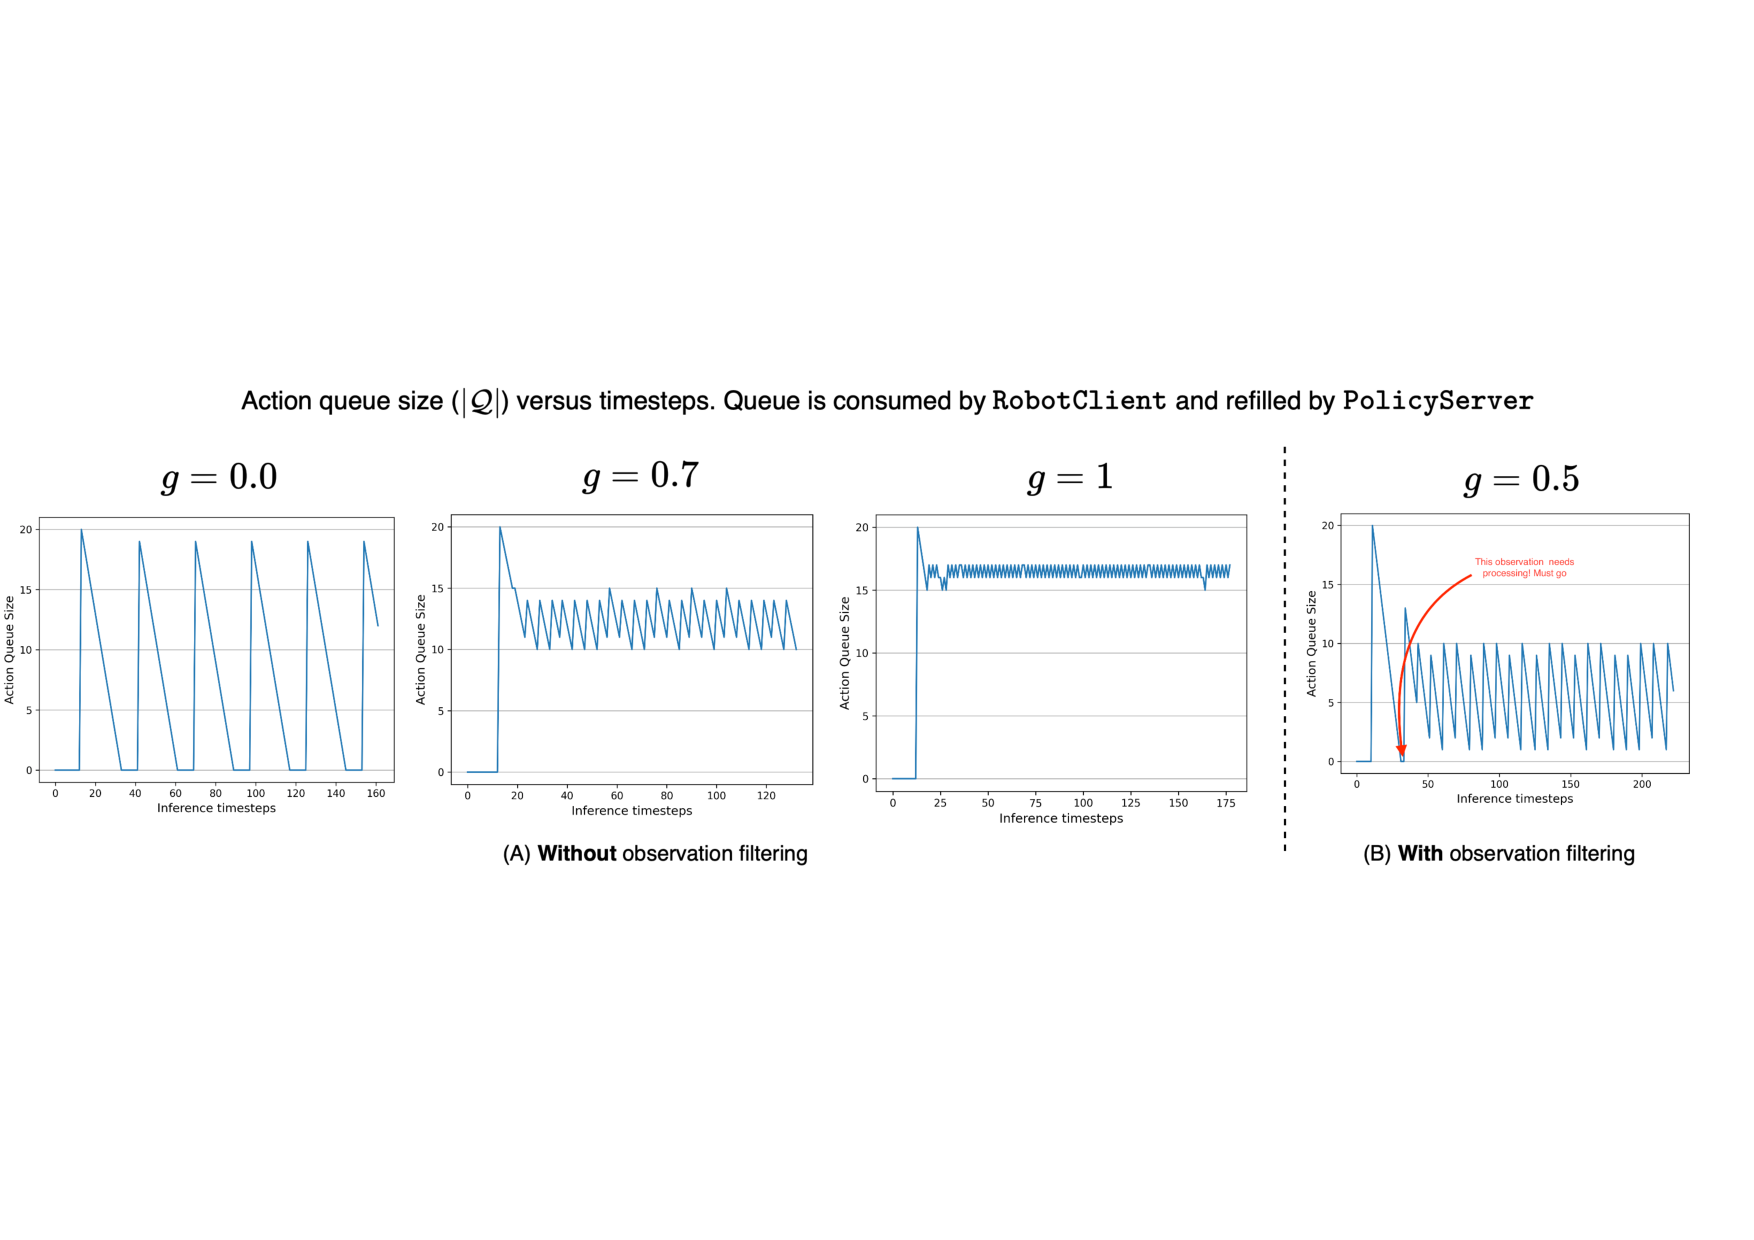
\includegraphics[width=\textwidth]{figures/queues.pdf}
        \caption{Action queue size evolution at runtime for various levels of \( g\) when (A) not filtering out observation based on joint-space similarity and (B) filtering out near-duplicates observation, measuring their similarity in joint-space.}
        \label{fig:queues}
    \end{minipage}
    % \vspace{-0.6cm}
\end{figure}

\Cref{fig:queues}(A) emphasizes the trade-off governed by \(g\): small values place result in idle periods, whereas \(g\approx 1\) assumes a highly accurate model and pays a significant compute price. In practice, choosing \(g\in(0,1)\) allows to strike a balance between reactivity against resource budgets. 
If not for the aforementioned similarity filter, the \textsc{RobotClient} would send observations for processing every \( (1 - g) n \cdot \Delta t\) seconds, receiving a new chunk of actions every \( (1 - g) n \cdot \Delta t + \mathbb E[\ell_S] \), on average. 
The presence of the observation similarity filter dilates this processing time, and serves the scope of avoiding the robot stalling due to the queue being constantly integrated with an incoming, nearly identical, action chunk. 
In particular, ~\Cref{fig:queues}(B) results in a queue which is filled with incoming actions \emph{unless} near-duplicate observations are filtered out from the processing pipeline. For clarity, the red arrow in \Cref{fig:queues}(B) highlights a timestep where the observation similarity mechanism is bypassed, forcing a (nearly identical) observation to be processed as the queue results empty.

%TODO(fracapuano): To extend this work, consider adding an analysis on how different the action queues produced are related to each other.